
%% bare_conf.tex
%% V1.3
%% 2007/01/11
%% by Michael Shell
%% See:
%% http://www.michaelshell.org/
%% for current contact information.
%%
%% This is a skeleton file demonstrating the use of IEEEtran.cls
%% (requires IEEEtran.cls version 1.7 or later) with an IEEE conference paper.
%%
%% Support sites:
%% http://www.michaelshell.org/tex/ieeetran/
%% http://www.ctan.org/tex-archive/macros/latex/contrib/IEEEtran/
%% and
%% http://www.ieee.org/

%%*************************************************************************
%% Legal Notice:
%% This code is offered as-is without any warranty either expressed or
%% implied; without even the implied warranty of MERCHANTABILITY or
%% FITNESS FOR A PARTICULAR PURPOSE! 
%% User assumes all risk.
%% In no event shall IEEE or any contributor to this code be liable for
%% any damages or losses, including, but not limited to, incidental,
%% consequential, or any other damages, resulting from the use or misuse
%% of any information contained here.
%%
%% All comments are the opinions of their respective authors and are not
%% necessarily endorsed by the IEEE.
%%
%% This work is distributed under the LaTeX Project Public License (LPPL)
%% ( http://www.latex-project.org/ ) version 1.3, and may be freely used,
%% distributed and modified. A copy of the LPPL, version 1.3, is included
%% in the base LaTeX documentation of all distributions of LaTeX released
%% 2003/12/01 or later.
%% Retain all contribution notices and credits.
%% ** Modified files should be clearly indicated as such, including  **
%% ** renaming them and changing author support contact information. **
%%
%% File list of work: IEEEtran.cls, IEEEtran_HOWTO.pdf, bare_adv.tex,
%%                    bare_conf.tex, bare_jrnl.tex, bare_jrnl_compsoc.tex
%%*************************************************************************

% *** Authors should verify (and, if needed, correct) their LaTeX system  ***
% *** with the testflow diagnostic prior to trusting their LaTeX platform ***
% *** with production work. IEEE's font choices can trigger bugs that do  ***
% *** not appear when using other class files.                            ***
% The testflow support page is at:
% http://www.michaelshell.org/tex/testflow/



% Note that the a4paper option is mainly intended so that authors in
% countries using A4 can easily print to A4 and see how their papers will
% look in print - the typesetting of the document will not typically be
% affected with changes in paper size (but the bottom and side margins will).
% Use the testflow package mentioned above to verify correct handling of
% both paper sizes by the user's LaTeX system.
%
% Also note that the "draftcls" or "draftclsnofoot", not "draft", option
% should be used if it is desired that the figures are to be displayed in
% draft mode.
%
\documentclass[10pt,journal,letterpaper,compsoc]{IEEEtran}
% Add the compsocconf option for Computer Society conferences.
%
% If IEEEtran.cls has not been installed into the LaTeX system files,
% manually specify the path to it like:
% \documentclass[conference]{../sty/IEEEtran}





% Some very useful LaTeX packages include:
% (uncomment the ones you want to load)


% *** MISC UTILITY PACKAGES ***
%
\usepackage{ifpdf}
% Heiko Oberdiek's ifpdf.sty is very useful if you need conditional
% compilation based on whether the output is pdf or dvi.
% usage:
% \ifpdf
%   % pdf code
% \else
%   % dvi code
% \fi
% The latest version of ifpdf.sty can be obtained from:
% http://www.ctan.org/tex-archive/macros/latex/contrib/oberdiek/
% Also, note that IEEEtran.cls V1.7 and later provides a builtin
% \ifCLASSINFOpdf conditional that works the same way.
% When switching from latex to pdflatex and vice-versa, the compiler may
% have to be run twice to clear warning/error messages.






% *** CITATION PACKAGES ***
%
%\usepackage{cite}
% cite.sty was written by Donald Arseneau
% V1.6 and later of IEEEtran pre-defines the format of the cite.sty package
% \cite{} output to follow that of IEEE. Loading the cite package will
% result in citation numbers being automatically sorted and properly
% "compressed/ranged". e.g., [1], [9], [2], [7], [5], [6] without using
% cite.sty will become [1], [2], [5]--[7], [9] using cite.sty. cite.sty's
% \cite will automatically add leading space, if needed. Use cite.sty's
% noadjust option (cite.sty V3.8 and later) if you want to turn this off.
% cite.sty is already installed on most LaTeX systems. Be sure and use
% version 4.0 (2003-05-27) and later if using hyperref.sty. cite.sty does
% not currently provide for hyperlinked citations.
% The latest version can be obtained at:
% http://www.ctan.org/tex-archive/macros/latex/contrib/cite/
% The documentation is contained in the cite.sty file itself.






% *** GRAPHICS RELATED PACKAGES ***
%
\ifCLASSINFOpdf
  % \usepackage[pdftex]{graphicx}
  % declare the path(s) where your graphic files are
  % \graphicspath{{../pdf/}{../jpeg/}}
  % and their extensions so you won't have to specify these with
  % every instance of \includegraphics
  % \DeclareGraphicsExtensions{.pdf,.jpeg,.png}
\else
  % or other class option (dvipsone, dvipdf, if not using dvips). graphicx
  % will default to the driver specified in the system graphics.cfg if no
  % driver is specified.
  % \usepackage[dvips]{graphicx}
  % declare the path(s) where your graphic files are
  % \graphicspath{{../eps/}}
  % and their extensions so you won't have to specify these with
  % every instance of \includegraphics
  % \DeclareGraphicsExtensions{.eps}
\fi
% graphicx was written by David Carlisle and Sebastian Rahtz. It is
% required if you want graphics, photos, etc. graphicx.sty is already
% installed on most LaTeX systems. The latest version and documentation can
% be obtained at: 
% http://www.ctan.org/tex-archive/macros/latex/required/graphics/
% Another good source of documentation is "Using Imported Graphics in
% LaTeX2e" by Keith Reckdahl which can be found as epslatex.ps or
% epslatex.pdf at: http://www.ctan.org/tex-archive/info/
%
% latex, and pdflatex in dvi mode, support graphics in encapsulated
% postscript (.eps) format. pdflatex in pdf mode supports graphics
% in .pdf, .jpeg, .png and .mps (metapost) formats. Users should ensure
% that all non-photo figures use a vector format (.eps, .pdf, .mps) and
% not a bitmapped formats (.jpeg, .png). IEEE frowns on bitmapped formats
% which can result in "jaggedy"/blurry rendering of lines and letters as
% well as large increases in file sizes.
%
% You can find documentation about the pdfTeX application at:
% http://www.tug.org/applications/pdftex





% *** MATH PACKAGES ***
%
%\usepackage[cmex10]{amsmath}
% A popular package from the American Mathematical Society that provides
% many useful and powerful commands for dealing with mathematics. If using
% it, be sure to load this package with the cmex10 option to ensure that
% only type 1 fonts will utilized at all point sizes. Without this option,
% it is possible that some math symbols, particularly those within
% footnotes, will be rendered in bitmap form which will result in a
% document that can not be IEEE Xplore compliant!
%
% Also, note that the amsmath package sets \interdisplaylinepenalty to 10000
% thus preventing page breaks from occurring within multiline equations. Use:
%\interdisplaylinepenalty=2500
% after loading amsmath to restore such page breaks as IEEEtran.cls normally
% does. amsmath.sty is already installed on most LaTeX systems. The latest
% version and documentation can be obtained at:
% http://www.ctan.org/tex-archive/macros/latex/required/amslatex/math/





% *** SPECIALIZED LIST PACKAGES ***
%
%\usepackage{algorithmic}
% algorithmic.sty was written by Peter Williams and Rogerio Brito.
% This package provides an algorithmic environment fo describing algorithms.
% You can use the algorithmic environment in-text or within a figure
% environment to provide for a floating algorithm. Do NOT use the algorithm
% floating environment provided by algorithm.sty (by the same authors) or
% algorithm2e.sty (by Christophe Fiorio) as IEEE does not use dedicated
% algorithm float types and packages that provide these will not provide
% correct IEEE style captions. The latest version and documentation of
% algorithmic.sty can be obtained at:
% http://www.ctan.org/tex-archive/macros/latex/contrib/algorithms/
% There is also a support site at:
% http://algorithms.berlios.de/index.html
% Also of interest may be the (relatively newer and more customizable)
% algorithmicx.sty package by Szasz Janos:
% http://www.ctan.org/tex-archive/macros/latex/contrib/algorithmicx/




% *** ALIGNMENT PACKAGES ***
%
%\usepackage{array}
% Frank Mittelbach's and David Carlisle's array.sty patches and improves
% the standard LaTeX2e array and tabular environments to provide better
% appearance and additional user controls. As the default LaTeX2e table
% generation code is lacking to the point of almost being broken with
% respect to the quality of the end results, all users are strongly
% advised to use an enhanced (at the very least that provided by array.sty)
% set of table tools. array.sty is already installed on most systems. The
% latest version and documentation can be obtained at:
% http://www.ctan.org/tex-archive/macros/latex/required/tools/


%\usepackage{mdwmath}
%\usepackage{mdwtab}
% Also highly recommended is Mark Wooding's extremely powerful MDW tools,
% especially mdwmath.sty and mdwtab.sty which are used to format equations
% and tables, respectively. The MDWtools set is already installed on most
% LaTeX systems. The lastest version and documentation is available at:
% http://www.ctan.org/tex-archive/macros/latex/contrib/mdwtools/


% IEEEtran contains the IEEEeqnarray family of commands that can be used to
% generate multiline equations as well as matrices, tables, etc., of high
% quality.


%\usepackage{eqparbox}
% Also of notable interest is Scott Pakin's eqparbox package for creating
% (automatically sized) equal width boxes - aka "natural width parboxes".
% Available at:
% http://www.ctan.org/tex-archive/macros/latex/contrib/eqparbox/





% *** SUBFIGURE PACKAGES ***
%\usepackage[tight,footnotesize]{subfigure}
% subfigure.sty was written by Steven Douglas Cochran. This package makes it
% easy to put subfigures in your figures. e.g., "Figure 1a and 1b". For IEEE
% work, it is a good idea to load it with the tight package option to reduce
% the amount of white space around the subfigures. subfigure.sty is already
% installed on most LaTeX systems. The latest version and documentation can
% be obtained at:
% http://www.ctan.org/tex-archive/obsolete/macros/latex/contrib/subfigure/
% subfigure.sty has been superceeded by subfig.sty.



%\usepackage[caption=false]{caption}
%\usepackage[font=footnotesize]{subfig}
% subfig.sty, also written by Steven Douglas Cochran, is the modern
% replacement for subfigure.sty. However, subfig.sty requires and
% automatically loads Axel Sommerfeldt's caption.sty which will override
% IEEEtran.cls handling of captions and this will result in nonIEEE style
% figure/table captions. To prevent this problem, be sure and preload
% caption.sty with its "caption=false" package option. This is will preserve
% IEEEtran.cls handing of captions. Version 1.3 (2005/06/28) and later 
% (recommended due to many improvements over 1.2) of subfig.sty supports
% the caption=false option directly:
%\usepackage[caption=false,font=footnotesize]{subfig}
%
% The latest version and documentation can be obtained at:
% http://www.ctan.org/tex-archive/macros/latex/contrib/subfig/
% The latest version and documentation of caption.sty can be obtained at:
% http://www.ctan.org/tex-archive/macros/latex/contrib/caption/




% *** FLOAT PACKAGES ***
%
%\usepackage{fixltx2e}
% fixltx2e, the successor to the earlier fix2col.sty, was written by
% Frank Mittelbach and David Carlisle. This package corrects a few problems
% in the LaTeX2e kernel, the most notable of which is that in current
% LaTeX2e releases, the ordering of single and double column floats is not
% guaranteed to be preserved. Thus, an unpatched LaTeX2e can allow a
% single column figure to be placed prior to an earlier double column
% figure. The latest version and documentation can be found at:
% http://www.ctan.org/tex-archive/macros/latex/base/



%\usepackage{stfloats}
% stfloats.sty was written by Sigitas Tolusis. This package gives LaTeX2e
% the ability to do double column floats at the bottom of the page as well
% as the top. (e.g., "\begin{figure*}[!b]" is not normally possible in
% LaTeX2e). It also provides a command:
%\fnbelowfloat
% to enable the placement of footnotes below bottom floats (the standard
% LaTeX2e kernel puts them above bottom floats). This is an invasive package
% which rewrites many portions of the LaTeX2e float routines. It may not work
% with other packages that modify the LaTeX2e float routines. The latest
% version and documentation can be obtained at:
% http://www.ctan.org/tex-archive/macros/latex/contrib/sttools/
% Documentation is contained in the stfloats.sty comments as well as in the
% presfull.pdf file. Do not use the stfloats baselinefloat ability as IEEE
% does not allow \baselineskip to stretch. Authors submitting work to the
% IEEE should note that IEEE rarely uses double column equations and
% that authors should try to avoid such use. Do not be tempted to use the
% cuted.sty or midfloat.sty packages (also by Sigitas Tolusis) as IEEE does
% not format its papers in such ways.





% *** PDF, URL AND HYPERLINK PACKAGES ***
%
%\usepackage{url}
% url.sty was written by Donald Arseneau. It provides better support for
% handling and breaking URLs. url.sty is already installed on most LaTeX
% systems. The latest version can be obtained at:
% http://www.ctan.org/tex-archive/macros/latex/contrib/misc/
% Read the url.sty source comments for usage information. Basically,
% \url{my_url_here}.


%my own packages
\usepackage{verbatim}
\usepackage{epsfig}
\usepackage{paralist}
\usepackage{algorithmic}
\usepackage{algorithm}
\usepackage{url}

%my own environment variables
\newtheorem{claim}{Claim}
\newtheorem{lemma}{Lemma}
\newtheorem{corollary}[lemma]{Corollary}
\newtheorem{definition}{Definition}
\newtheorem{observation}{Observation}
\newtheorem{constraint}{Constraint}

\def\colrule{\\[-7pt]\hline\\[-6pt]}


\makeatletter
\def\imod#1{\allowbreak\mkern10mu({\operator@font mod}\,\,#1)}
\makeatother
% *** Do not adjust lengths that control margins, column widths, etc. ***
% *** Do not use packages that alter fonts (such as pslatex).         ***
% There should be no need to do such things with IEEEtran.cls V1.6 and later.
% (Unless specifically asked to do so by the journal or conference you plan
% to submit to, of course. )


% correct bad hyphenation here
\hyphenation{op-tical net-works semi-conduc-tor}


\begin{document}


%
% paper title
% can use linebreaks \\ within to get better formatting as desired
\title{
%Improving the scalability of protein sequence clustering for large-scale metagenomic data sets
{\it pGraph}: Constructing Large-Scale Protein Sequence Homology Graphs Efficiently on Distributed Memory Machines
}


% author names and affiliations
% use a multiple column layout for up to two different
% affiliations
\author{Changjun Wu,
        Ananth Kalyanaraman,
        and William R. Cannon% <-this % stops a space
\IEEEcompsocitemizethanks{\IEEEcompsocthanksitem C. Wu and A. Kalyanaraman are with the School of Electrical Engineering and Computer Science, Washington State University, Pullman, WA, 99164.\protect\\
% note need leading \protect in front of \\ to get a newline within \thanks as
% \\ is fragile and will error, could use \hfil\break instead.
E-mail: \{cwu2, ananth\}@eecs.wsu.edu
\IEEEcompsocthanksitem W.R Cannon is with Pacific Northwest National Laboratory, Richland, WA. 99352.\protect\\
E-mail: william.cannon@pnl.gov}
\thanks{}}

% conference papers do not typically use \thanks and this command
% is locked out in conference mode. If really needed, such as for
% the acknowledgment of grants, issue a \IEEEoverridecommandlockouts
% after \documentclass

% for over three affiliations, or if they all won't fit within the width
% of the page, use this alternative format:
% 
%\author{\IEEEauthorblockN{Michael Shell\IEEEauthorrefmark{1},
%Homer Simpson\IEEEauthorrefmark{2},
%James Kirk\IEEEauthorrefmark{3}, 
%Montgomery Scott\IEEEauthorrefmark{3} and
%Eldon Tyrell\IEEEauthorrefmark{4}}
%\IEEEauthorblockA{\IEEEauthorrefmark{1}School of Electrical and Computer Engineering\\
%Georgia Institute of Technology,
%Atlanta, Georgia 30332--0250\\ Email: see http://www.michaelshell.org/contact.html}
%\IEEEauthorblockA{\IEEEauthorrefmark{2}Twentieth Century Fox, Springfield, USA\\
%Email: homer@thesimpsons.com}
%\IEEEauthorblockA{\IEEEauthorrefmark{3}Starfleet Academy, San Francisco, California 96678-2391\\
%Telephone: (800) 555--1212, Fax: (888) 555--1212}
%\IEEEauthorblockA{\IEEEauthorrefmark{4}Tyrell Inc., 123 Replicant Street, Los Angeles, California 90210--4321}}




% use for special paper notices
%\IEEEspecialpapernotice{(Invited Paper)}

% for Computer Society papers, we must declare the abstract and index terms
% PRIOR to the title within the \IEEEcompsoctitleabstractindextext IEEEtran
% command as these need to go into the title area created by \maketitle.
\IEEEcompsoctitleabstractindextext{%
\begin{abstract}
%\boldmath
Protein sequence homology detection is a fundamental problem in computational molecular biology, with a pervasive application in nearly all analyses that aim to structurally and functionally characterize protein molecules. While detecting homology between two protein sequences is computationally inexpensive, detecting pairwise homology at a large-scale becomes prohibitive, requiring millions of CPU hours. Yet, there is currently no efficient method available to parallelize this kernel. In this paper, we present the key characteristics that make this problem particularly hard to parallelize, and then propose a new parallel algorithm that is suited for large-scale protein sequence data. Our method, called {\it pGraph}, is designed using a hierarchical multiple-master multiple-worker model, where the processor space is partitioned into subgroups and the hierarchy helps in ensuring the workload is load balanced fashion despite the inherent irregularity that may originate in the input. Experimental evaluation demonstrates that our method scales linearly on all input sizes tested (up to 640K sequences) on a 1,024 node supercomputer. In addition to demonstrating strong scaling, we present an extensive study of the various components of the system and related parametric studies. 
\end{abstract}
% IEEEtran.cls defaults to using nonbold math in the Abstract.
% This preserves the distinction between vectors and scalars. However,
% if the journal you are submitting to favors bold math in the abstract,
% then you can use LaTeX's standard command \boldmath at the very start
% of the abstract to achieve this. Many IEEE journals frown on math
% in the abstract anyway. In particular, the Computer Society does
% not want either math or citations to appear in the abstract.

% Note that keywords are not normally used for peer review papers.
\begin{keywords}
Parallel protein sequence homology detection; parallel sequence graph construction; hierarchical master-worker paradigm.
\end{keywords}}


% make the title area
\maketitle

% For peer review papers, you can put extra information on the cover
% page as needed:
% \ifCLASSOPTIONpeerreview
% \begin{center} \bfseries EDICS Category: 3-BBND \end{center}
% \fi
%
% For peerreview papers, this IEEEtran command inserts a page break and
% creates the second title. It will be ignored for other modes.
\IEEEpeerreviewmaketitle

\section{Introduction}
\label{secIntroduction}

Protein sequence homology detection is a fundamental problem in computational molecular biology, where given a set of protein sequences, the goal is to identify \emph{highly similar pairs of sequences}. In graph-theoretic terms, if we were to represent the input protein sequences as vertices and pairwise sequence similarity as edges, then the problem of pairwise homology detection is equivalent of constructing the graph. 

Homology detection is widely used in nearly all analyses targeted at functional and structural characterization of protein molecules \cite{Kriventseva01}. Most notably, the operation is heavily used in clustering applications, where the problem is to partition the input sequences such that all proteins that are ``related'' to one another by a pre-defined degree of sequence homology are grouped together. 
%In graph-theoretic terms, if we were to represent the input protein sequences as vertices and pairwise sequence similarity as edges, then the problem of clustering is to find maximal cliques. In practice, however, owing to errors in sequence data and other biological considerations (e.g., functionally related proteins could differ at the sequence level), the problem is one of finding dense subgraphs \cite{Yooseph07}. 
Clustering has become highly significant of late because of its potential to uncover thousands of previously unknown proteins from metagenomic data sets. Metagenomics \cite{Handelsman04}, which is a rapidly emerging sub-field, involves the study of environmental microbial communities using novel genomic tools. In 2007, a single study that surveyed an ocean microbiota \cite{Yooseph07} resulted in the discovery of nearly $4\times 10^3$ previously unknown protein families, significantly expanding the protein universe as we know it. As protein families are defined as groups of functionally related proteins, homology detection and clustering play a central role during family identification. 

While there are numerous software options available for protein sequence clustering (e.g., \cite{Apweiler04,Bateman04,Enright02,Kriventseva01,Olman07}), all of them assume that the graph is already constructed and available as input. However, modern-day use-cases such as the ocean metagenomic sequence clustering suggest that this is not the case. This is because these large-scale projects generate sequence information of their own and hence will have to contend with detecting the sequence homology among all new sequences and against sequence information generated from previous projects. For example, the ocean metagenomic project alone generated more than 17 million new protein (ORF) sequences and this set was analyzed alongside over 11 million  sequences downloaded from public protein sequence databanks (for a total of 28.6 million sequences). Consequently, the most dominant phase of computation in the entire analysis was the detection of pairwise sequence homology, which alone took $10^6$ CPU hours, even after using heuristic approaches to compute homology \cite{Yooseph07}. Our own experience with the homology detection phase \cite{Wu08} is further confirmation for the challenges that confront this problem.

In this paper, we propose a new parallel algorithm for carrying out sequence homology detection of 
large-scale protein sequence data. Through detection, the resulting output is the sequence graph which can be directly used as input for the subsequent clustering step.

Developing a scalable solution for this problem using parallel processing is essential for this emerging application domain as it can help reduce the time to solution and enable larger data sets to be analyzed. The problem also has several attributes that make it interesting from the standpoint of parallel algorithm development. (i) {\bf Input size:} Firstly, the problem is data-intensive. Tens of millions of protein sequences are already available from public repositories (e.g., CAMERA \url{http://camera.calit2.net/}). (ii) {\bf Work processing rate:} The rate at which work is processed could be highly irregular. Detecting pairwise sequence homology is equivalent to the problem of finding optimal alignment \cite{Smith81}, the time for which is proportional to the product of lengths of the strings being aligned. However, due to the large variance in the input protein sequence length, the time to process each unit of work could also vary significantly, as will be shown in Section~\ref{secResults}.  (iii) {\bf Work generation rate:} To avoid a brute-force all-against-all sequence comparison, a string index such as suffix tree \cite{Weiner73} or look-up table \cite{Altschul90} is used so that only pairs satisfying an exact matching criterion need to be further evaluated \cite{Wu08, Yooseph07}. However, the rate at which the pairs are generated could be irregular. For instance, same sized portions of the suffix tree index could result in the generation of drastically different number of sequence pairs for alignment, as will be shown in Section~\ref{secResults}. {\it A priori} stocking of pairs that require alignment is also not an option because of a worst-case quadratic explosion of work. (iv) {\bf Local availability of data:}  Finally, the ready in-memory availability of sequence data during alignment processing cannot be guaranteed under distributed memory machine setting because of large input sizes. Alternatively, moving computation to data is also virtually impossible because a pair listed for alignment work could involve any two input sequence. The algorithm proposed in this paper addresses all these challenges.


\subsection{Contributions}
\label{secContributions}

In this paper, we present a novel algorithm for carrying out large-scale protein sequence homology detection. Our algorithm, called {\it pGraph}\footnote{stands for ``\underline{p}rotein sequence homology \underline{Graph} construction''}, is designed to take advantage of the large-scale memory and compute power available from distributed memory parallel machines. The method uses a hierarchical multiple-master multiple-worker model to dynamically distribute tasks corresponding to both work generation and work processing in a load balanced fashion. The processor space is organized into subgroups with each subgroup consisting of a producer (for work generation), a master (for work distribution) and a fixed number of workers acting as consumers of work. This producer-consumer model of organizing a subgroup helps decouple work generation from work processing. In addition, a dedicated supermaster is tasked with the responsibility of ensuring that the tasks are evenly shared among subgroups. The multiple-master model also helps avoid single point bottlenecks.

Experimental results show that this new approach achieves linear scaling on 1,024 nodes for the range of input tested (up to 640,000 sequences). More notably, the method was able to maintain parallel efficiency at more than 90\% over all processor size tested. In addition to scalability results, we also present a thorough report on the system behavior by components. Though presented in the context of protein sequence graph construction, our method could be extended to other data-intensive applications where there is irregularity in work generation and/or in work processing. 

The paper is organized as follows. Section~\ref{secRelatedWork} presents the current state of art for parallel sequence homology detection. Section~\ref{secMethods} presents our proposed method and implementation details. Experimental results are presented and discussed in Section~\ref{secResults}, and Section~\ref{secConclusions} concludes the paper.




\section{Related Work}
\label{secRelatedWork}

Sequence homology between two protein sequences can be evaluated using rigorous optimal alignment algorithms \cite{Needleman70,Smith81} or heuristic alignment methods such as BLAST \cite{Altschul90}. Protein sequence clustering is a well researched topic with numerous algorithms and software tools (e.g., \cite{Apweiler04,Bateman04,Enright02,Kriventseva01,Olman07}). While sequence homology is a fundamental computational kernel within clustering applications, there are currently no efficient parallel algorithms. In order to accommodate for the $10^6$ CPU hours, the ocean metagenomics project \cite{Yooseph07} used an {\it ad hoc} parallel strategy, where an all-against-all sequence comparison using BLAST was manually partitioned across 125 dual processors systems and 128 16-processor nodes each containing between 16GB-64GB of RAM. 

Recently, we proposed a parallel method \cite{Wu08} for the problem of protein clustering. The main contribution of this method was that it showed how to break a single large graph problem into multiple disjoint subproblems. This was achieved by first enumerating all connected components so that the individual components can be post-processed independently for dense subgraph detection. However, detecting connected components also involves enumerating all the edges of the graph through sequence homology detection. While performance tests demonstrated linear scaling up to 128 processors for 160,000 sequences, the phase for pairwise sequence homology detection failed to scale linearly for larger number of processors \cite{Wu08}. The cause for the slowdown was primarily the irregularity that was observed between pair generation and alignment computation. Interestingly, the same scheme had demonstrated linear scaling on DNA sequence clustering problems earlier \cite{Kalyanaraman07}. This is the motivation behind our newly proposed design which decouples the work generation (producer) from work processing (consumer).

Our observations of a higher complexity for metagenomic protein data when compared to DNA data are consistent with other previous studies. For example, in the human genome assembly project \cite{Venter01}, the all-against-all sequence homology detection of roughly 28 million DNA sequences consumed only $10^4$ CPU hours. Contrast this with the $10^6$ CPU hours observed for analyzing roughly the same number of protein sequences in the ocean metagenomic project \cite{Yooseph07}.


\section{Methods}
\label{secMethods}

\noindent{\bf Notation:} Let $S=\{s_1,s_2,\ldots s_n\}$ denote the set of $n$ input protein sequences, and Let $p$ denote the set of processors. Let $G=(V,E)$ denote a graph defined as $V=S$ and $E=\{(s_i,s_j)$ $|$ $s_i$ and $s_j$ have a significant sequence similarity\}.\\

\noindent{\bf Problem statement:} Given a set $S$ of $n$ protein sequences and $p$ processors, the protein sequence graph construction problem is to construct $G$ in parallel.\\

Given $S$, the primary question is to detect if there exists an edge between any two vertices. While it is computationally inexpensive to determine an optimal alignment between two average-length protein sequences, performing hundreds of millions to billions of alignment computations could be highly prohibitive (e.g., \cite{Wu08, Yooseph07}).  There are two independent ways to reduce the computational burden --- one is to use algorithmic heuristics (see Section~\ref{secGeneratingPairs}) and another is to use high performance computing (see Section~\ref{secMasterSlave}).

%\subsection{Computin}
%\label{secAlgorithm}



\begin{figure}[tb]
\centerline{
						%\scalebox{0.7}{\input{figFramework.pstex_t}}
						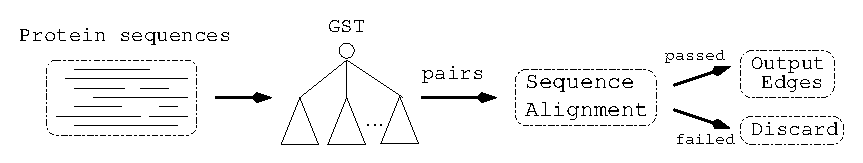
\includegraphics[angle=0, scale=0.60]{icppFram.eps}
            }
\caption{
Tree-based filtering scheme used by our approach for protein sequence homology detection. $GST$ stands for Generalized Suffix Tree.
}
\label{figFramework}
\end{figure}

\subsubsection{Generating pairs}
\label{secGeneratingPairs}

A brute-force approach to detect the presence of an edge is to enumerate all possible pairs of sequences and retain only those as edges which pass the alignment test. Such an approach would evaluate $n\choose 2$ pairs for alignment, and hence is not a scalable solution. Alternatively, since alignments represent approximate matching, the presence of long exact matches can be used as a necessary but not sufficient condition \cite{Kalyanaraman07}. This approach can filter out a significant fraction of poor quality pairs and thereby reduce the number of pairs aligned significantly (e.g., by $>70\%$ \cite{Wu08}).  Figure~\ref{figFramework} illustrates the tree based filtering scheme.

To implement exact matching, we use the maximal match detection algorithm described in \cite{Kalyanaraman07}. This method generates only those pairs that show high promise for passing the alignment test. It first builds a Generalized Suffix Tree (GST) data structure \cite{Weiner73} as a string index for the strings in $S$. The tree index is generated as a forest of subtrees and then the individual subtrees are traversed to generate pairs. The pair generation process may exhibit nonuniformity in the sense that subtrees with the similar size could produce drastically different number of pairs and/or at different rates (as shown in Section~\ref{secResults}). This is because the composition of a subtree is purely data-dependent and if a section of subtree receives a highly repetitive fraction of the input sequences then it is bound to generate a disproportionately large number of pairs. The tree construction code outputs the GST as a forest of subtrees on to the file system, with a small fixed number of sub-trees in each file.


%\subsubsection{Computing an alignment}
%\label{secAlignments}

%A pair of sequences $(s_i,s_j)$ short-listed by the pair generation algorithm are evaluated using the Smith-Waterman algorithm. For scoring amino acid substitutions between the two protein sequences, our default implementation uses a user-specified substitution matrix such as BLOSUM62 \cite{Henikoff92}. For alignment criteria, we use the same parameters described in \cite{Wu08, Yooseph07}. If a pair passes this alignment test, then it is output as an edge into a file. Furthermore, an additional check is performed to see if one of the sequences in the pair is contained within the other sequence, and if so, it is marked as a ``redundant sequence'' and output to another file. 


\subsection{{\it pGraph}: Parallel graph construction}
\label{secMasterSlave}



\begin{figure}[tb]
\centerline{
						\scalebox{0.65}{\input{figPClust.pstex_t}}
            }
\caption{
The hierarchical multiple-master multiple-worker design of the {\it pGraph} approach showing the interaction of the individual components within and outside the subgroups.
}
\label{figPClust}
\end{figure}

In this section, we present a novel and efficient parallel algorithm to compute sequence alignments on the pairs generated from the tree index and output edges of the graph $G$. Our method uses a hierarchical multiple-master multiple-worker model to counter the challenges posed by inherent irregularities of pair generation and alignment rates. 

The system architecture is illustrated in Figure~\ref{figPClust}. The inputs include the sequence set $S$ and the tree index $T$. The tree index is available as a forest of $k$ subtrees, which we denote as $T=\{t_1,t_2,\ldots t_k\}$. In both theory and practice, the value of $k$ tends to be of the order of $n$, which is good for parallel distribution for large values of $n$. The output of {\it pGraph} is the set of all edges of the form $(s_i,s_j)$ s.t., the sequences $s_i$ and $s_j$ pass the alignment test based on user-defined cutoffs. Given $p$ processors and a small number $q\geq 3$, the parallel system is partitioned as follows: i) one processor is designated to act as the \emph{supermaster} for the entire system; and ii) the remaining $p-1$ processors are partitioned into $m$ subgroups such that each subgroup has exactly $q$ processors\footnote{With the possible exception of one subgroup which may obtain less than $q$ processors if $(p-1)\%q\ne 0$.}. Furthermore, a subgroup is internally organized with one processor designated to the role of a \emph{producer}, another to the role of a \emph{master}, and the remaining $q-2$ processors to the role of a \emph{consumer}. 

At a high level, the producers are responsible for pair generation, the masters for distributing the alignment workload within their respective subgroups, and the consumers for computing alignments. The supermaster plays a supervisory role to ensure load is distributed evenly among subgroups. Nevertheless, there are several design considerations that need to be taken into account. In what follows, we explain these factors and present algorithms and protocols for each component in the system. 

\noindent{\bf Notation: } Let:\\
%\begin{itemize}\itemsep=-0.05ex
$P_{buf}\leftarrow$ a fixed sized pair buffer at the producer;\\
$M_{buf}\leftarrow$ a fixed sized pair buffer at the master;\\
$C_{buf}\leftarrow$ a fixed sized pair buffer at the consumer;\\
$S_{buf}\leftarrow$ a fixed sized pair buffer at the supermaster;\\
$b_1\leftarrow$ batch size (for pairs) from producer or supermaster to master;\\
$b_2\leftarrow$ batch size (for pairs) from master to consumer;\\


\noindent{\bf Producer: }
The primary responsibility of a producer is to load a subset of subtrees in $T$ and generate pairs using the maximal matching algorithm in \cite{Kalyanaraman07}. Pairs could be allocated for alignment computation by communicating them to the local master in the subgroup and have the master assign pairs to its consumers. However, such an approach runs the risk of a potential bottleneck situation where a producer receives a subtree that generates a significantly large volume of pairs and/or generate pairs that take significantly long alignment times. Another issue is the timing of communicating the pairs for alignment allocation. The memory limitation at the producer limits the size of $P_{buf}$ used for temporary pair storage. On the other hand, immediately dispatching the pairs as they are generated may increase communication overhead or may overrun $M_{buf}$. Assigning subtrees to producers will also have to be done dynamically at a fine granular level as otherwise it may result in nonuniform distribution of pairs across subgroups. 

To overcome the above challenges, the algorithm shown in Algorithm~\ref{pd} is followed. Initially, a producer fetches a batch of subtrees (available as a single file) from the supermaster. The producer then starts to generate and enqueue pairs into $P_{buf}$. Subsequently, the producer dequeues and sends $b_1$ pairs to the master. This is implemented using a nonblocking send so that when the master is not yet ready to accept pairs, the producer can continue to generate pairs, thereby allowing masking of communication. After processing the current batch of subtrees, the producer requests another batch from the supermaster. Once there are no more subtrees available, the producers dispatch pairs to both master \emph{and} supermaster, depending on whoever is responsive to their nonblocking sends. This strategy gives the producer an option of redistributing its pairs to other subgroups (via supermaster) if the local master is busy. In fact, we show in the experimental section that the strategy of using the supermaster route pays off significantly and ensures the system is load balanced. \\

\begin{algorithm}
\caption{Producer}
\label{pd}
\algsetup{
  linenosize=\small,
  linenodelimiter=.
}
\begin{algorithmic}[1]
    \STATE Request a batch of subtrees from supermaster
    \WHILE{\TRUE}
        \STATE $T_i \leftarrow$ received subtrees from supermaster 
        \IF{$T_i = \emptyset$}
            \STATE {break while loop}
        \ENDIF
        \REPEAT
            \IF{$P_{buf}$ is not FULL}
                \STATE Generate at most $b_1$ pairs from $T_i$
                \STATE Insert new pairs into $P_{buf}$
            \ENDIF
            \IF{$send_{P\rightarrow M}$ completed}
                \STATE Extract at most $b_1$ pairs from $P_{buf}$
                \STATE $send_{P\rightarrow M}\leftarrow$ {\it Isend} extracted pairs to master
            \ENDIF
        \UNTIL{$T_i = \emptyset$}
        \STATE Request a batch of subtrees from supermaster
    \ENDWHILE
    \STATE /* Flush remaining pairs */
    \WHILE {$P_{buf} \neq \emptyset$}
        \STATE Extract at most $b_1$ pairs from $P_{buf}$
        \IF{$send_{P\rightarrow M}$ completed}
            \STATE $send_{P\rightarrow M}\leftarrow$ {\it Isend} extracted pairs to master
        \ENDIF
        \IF{$send_{P\rightarrow S}$ completed}
            \STATE $send_{P\rightarrow S}\leftarrow$ {\it Isend} extracted pairs to supermaster
        \ENDIF
    \ENDWHILE
    \STATE Send END signal to supermaster
\end{algorithmic}
\end{algorithm}


\noindent{\bf Master: }
The primary responsibility of a master is to ensure all consumers in its subgroup are always busy with alignment computation. The main challenge in this setup is to ensure that a master's local buffer for storing pairs ($M_{buf}$) is not overrun by an overactive producer or is starved due to a slow producer. Either of these could happen because the pair generation rate is data-dependent. The above challenge is overcome as follows (see Algorithm~\ref{ms}).  

Initially, to ensure that there is a steady supply and dispatch of pairs, the master listens for messages from both its producer and consumers. However, once $|M_{buf}|$ reaches a preset limit called $\tau$, the master realizes that its producer has been more active than the rate at which pairs are processed at its consumers, and therefore shuts off listening to its producer, while only dispatching pairs to its consumers until $|M_{buf}|\leq\tau$. The rationale for this strategy is the practical expectation that pair generation tends to happen much faster than pair alignment. More importantly, this strategy helps to keep the consumers always busy with alignment computation. Since consumers are the majority in the system, this has a direct scalability implication. When the  producer has exhausted sending all its pairs, the master can fallback on the supermaster to provide pairs. 

As for serving consumers, the master maintains a priority queue, which keeps track of each of its consumers based on the latter's most recent status report to the master. Priority is defined based on the number of pairs left to be processed at the consumer's $C_{buf}$. Priority is implemented in the master as follows: at any given iteration, pairs are allocated in batches of size $b_2$ and send to consumers in the decreasing (or, nonincreasing) order of priority. While frequent updates from consumers could help the master to better assess the situation on each consumer, such a scheme will also increase communication overhead. As a tradeoff, we implement a priority queue by maintaining only three levels of priority depending on the condition of a consumer's $C_{buf}$: $\frac{1}{2}$-empty, $\frac{3}{4}$-empty, and completely empty. This also implies that the master, instead of pushing pairs on to consumers, waits for consumers to take the initiative in requesting pairs, while reacting in the order of their current workload status. \\







\begin{algorithm}
\caption{Master}
\label{ms}
\algsetup{
  linenosize=\small,
  linenodelimiter=.
}
\begin{algorithmic}[1]

    \STATE $\tau$: predetermined cutoff for the size of $M_{buf}$
    %\STATE $C=\{c_1, c_2, ...\}$: consumers in the subgroup
    \STATE $Q$: priority queue for consumers

    \WHILE{\TRUE}
        \STATE /* Recv messages */
        \IF{$|M_{buf}| > \tau$}
            \STATE $msg\leftarrow$ post {\it Recv} for consumers
        \ELSE 
            \STATE $msg\leftarrow$ post open {\it Recv}
            \IF {$msg \equiv$ pairs}
                \STATE Insert pairs into $M_{buf}$
                \IF {$msg \equiv$ END signal from supermaster}
                    \STATE {break while loop}
                \ENDIF
            \ELSIF {$msg \equiv$ request from consumer}
                \STATE Place consumer in the appropriate priority queue
            \ENDIF
        \ENDIF
        
        \STATE /* Process consumer requests */
        \WHILE {$|M_{buf}|>0$ \AND $|Q|>0$}
            \STATE Extract a highest priority consumer, and send appropriate amount of pairs
        \ENDWHILE
    \ENDWHILE
    \STATE /* Flush remaining pairs to consumers */
    \WHILE{$|M_{buf}|>0$}
             \IF {$|Q|>0$}
                \STATE Extract a highest priority consumer, and send appropriate amount of pairs
            \ELSE
                \STATE Waiting consumer requests
            \ENDIF
    \ENDWHILE
    \STATE Send END signal to consumers
\end{algorithmic}
\end{algorithm}



\noindent{\bf Consumer: }
The primary responsibility of the consumer is to compute optimal alignments using the Smith-Waterman algorithm \cite{Smith81} for the pairs allocated to it by its master and output results. The main challenge is to ensure that a consumer does not starve for work. The consumer follows Algorithm~\ref{cs}. The consumer maintains a fixed size pair buffer $C_{buf}$. When the master sends a new batch of $b_2$ pairs, it starts processing them one at a time. When $C_{buf}$ reaches half size, the consumer sends out a message to the master updating its new buffer status, and continues processing of the remaining pairs in $C_{buf}$. At this stage, it also posts a nonblocking receive to accept new pairs from master while it is computing alignments. The send is also implemented as nonblocking to allow for further communication masking. Another message is sent out at the $\frac{1}{4}$ stage, but only after checking the status of the previous receive. If the master had sent pairs in the meantime, then the pairs are inserted into $C_{buf}$ and the processing continues. Alternatively, if there were no messages from the master and $C_{buf}$ becomes empty, the consumer sends another message to inform the master that it is starving and waits for the master to reply.

Before aligning a batch of pairs, the consumer has to ensure that the sequences needed are available in the local memory. While the local memory on a consumer may not be always sufficient to store the entire set of input sequences ($S$), it could be used to cache many strings. We use a parameter $\psi \leq n$ for this purpose. At initialization, all consumers load an arbitrary collection $\psi$ sequences from I/O. This statically allocated buffer is then used as a string cache during alignment computation. Only strings which are not in the local cache are fetched from I/O.\\


\begin{algorithm}
\caption{Consumer}
\label{cs}
\algsetup{
  linenosize=\small,
  linenodelimiter=.
}
\begin{algorithmic}[1]
    \STATE $g$: number of consumers in the same subgroup
    \STATE $\psi=\frac{n}{g}$: number of sequences to be cached statically
    \STATE {EMPTY, HALF, QUARTER}: $0$, $\frac{b_2}{2}$ and $\frac{b_2}{4}$ buffer status
    \STATE $S_{cache}\leftarrow$ load $\psi$ sequences from I/O
      
    \STATE $Recv\leftarrow$post nonblocking receive
    \WHILE {\TRUE}
    	    \IF {{$Recv$} completed}
            	\IF {Sequence request from consumer $c_{k}$}
			\STATE Pack sequences and send them out to $c_{k}$
			\STATE $Recv\leftarrow$post nonblocking receive
            	\ELSIF {Sequences from other consumer}
			\STATE Unpack sequences to dynamically cache
			\STATE $Recv\leftarrow$post nonblocking receive
            	\ELSIF {Pairs from master}
		        \STATE Insert pairs into $C_{buf}$
			\STATE Prepare sequence requests for each consumer
			\STATE Send sequence requests to other consumers
			\STATE $Recv\leftarrow$post nonblocking receive
	        \ENDIF
	    \ELSE
	    	\IF {$C_{buf} > 0$}
			\STATE /* Align a pair if their seqs. are ready */
	    		\STATE extract next pair $(i, j)$ from $C_{buf}$
			\IF {both $s_i$ and $s_j$ are ready}
				\STATE Align sequences $s_{i}$ and $s_{j}$
			\ELSE
				\STATE Append pair $(i, j)$ at the end of the $C_{buf}$
			\ENDIF
			
			\STATE /* Report $C_{buf}$ status back to master */
			\IF {$C_{buf}$=$\frac{b_2}{2}$}
				\STATE Send HALF status to master
			\ELSIF {$C_{buf}$=$\frac{b_2}{4}$}
				\STATE Send {\bf QUARTER} status to master
			\ELSIF {$C_{buf}= 0$}
				\STATE Send {\bf EMPTY} status to master
			\ENDIF
		\ENDIF
            \ENDIF
    \ENDWHILE
\end{algorithmic}
\end{algorithm}





\noindent{\bf Supermaster: }
The primary responsibility of the supermaster is to ensure both the pair generation workload and pair alignment workload are balanced across subgroups. To achieve this, the supermaster follows Algorithm~\ref{sp}. At any given iteration, the supermaster is either serving a producer or a master. For managing the pair generation workload, the supermaster assumes the responsibility of distributing subtrees (in batches) to individual producers. The supermaster, instead of pushing subtree batches to producers, waits for producers to request for the next batch. This approach guarantees that the run-time among producers, and not the number of subtrees processed, is balanced at program completion. 

The second task of the supermaster is to serve as a conduit for pairs to be redistributed across subgroup boundaries. To achieve this, the supermaster maintains a local buffer, $S_{buf}$. Producers can choose to send pairs to supermaster if their respective subgroups are saturated with alignment work. The supermaster then decides to push the pairs (in batches of size $b_1$) to masters of other subgroups, depending on their respective response rate (dictated by their current workload). This functionality is expected to be brought into effect at the ending stages of producers' pair generation, when there could be a few producers that are still churning out pairs in numbers while other producers have completed generating pairs. As a further step toward ensuring load balanced distribution at the producers' ending stages, the supermaster sends out batches of a reduced size, $\frac{b_1}{2}$, in order to compensate for the deficiency in pair supply. Correspondingly, the masters also reduce their batchsizes proportionately at this stage. As will shown in our experimental section, the supermaster plays a key role in load balancing of the entire system.



\begin{algorithm}
\caption{Supermaster}
\label{sp}
\algsetup{
  linenosize=\small,
  linenodelimiter=.
}
\begin{algorithmic}[1]
	\STATE Let $P=\{p_1, p_2, ...\}$ be the set of active producers
	\STATE $Recv_{S\leftarrow P}\leftarrow$ Post a nonblocking receive for producers
		\WHILE{$|P| \neq 0$}
			
	    
	    \STATE /* Serve the masters*/        
	     \IF{$|S_{buf}| > 0$}
	    	
	    	\STATE $m_i\leftarrow$ Select master for pairs allocation
		    \STATE Extract and {\it Isend} $b_1$ pairs to $m_i$ 
		    	
		    \ENDIF
		   	%\IF{$S_{buf}$ is FULL}
		    %    \STATE go to next iteration
		    %	\ENDIF	    
		    \STATE /* Serve the producers*/        
		    \IF{$Recv_{S\leftarrow P}$ completed}
		        \IF{$msg\equiv$ subtree request}
		             \STATE Send a batch of subtrees ($T_i$) to corresponding producer
		        \ELSIF{$msg\equiv$ pairs} 
			        \STATE Insert pairs in $S_{buf}$
		        \ENDIF
		        \STATE $Recv_{S\leftarrow P}\leftarrow$ Post a nonblocking receive for producers
		    \ENDIF
	    
	    
    \ENDWHILE

	\STATE Distribute remaining pairs to all masters in a round-robin way
	\STATE Send END signal to all masters
\end{algorithmic}
\end{algorithm}


\subsection{Implementation}
The {\it pGraph} code was implemented in C/MPI. All parameters described in the algorithm section were set to values based on preliminary empirical tests.  The default settings are as follows: $b_1=$30,000; $b_2=$2,000; $|P_{buf}|=5\times 10^7$; $|M_{buf}|=6\times 10^4$; $|C_{buf}|=6\times 10^3$; $|S_{buf}|=4\times 10^6$. 


\section{Experimental Results \& Discussion}
\label{secResults}


\subsection{Experimental setup} 

{\bf Input data:} The {\it pGraph} implementations were tested using an arbitrary collection of $2.56\times 10^6$ ($n$) amino acid sequences representing an ocean metagenomic data set available at the CAMERA metagenomics data archive \cite{}. The sum of the length of the sequences ($m$) in this set is 390,345,218, and the mean$\pm\sigma$ is $152.48\pm 167.25$; the smallest sequence has 1 residues and longest 32,794 residues. Smaller size subsets containing 20K, 40K, 80K, $\ldots$, $1.28\times 10^6$  were derived and used for scalability tests.

\noindent{\bf Experimental platform: } All tests were performed on the {\it Chinook} supercomputer at the EMSL facility in Pacific Northwest National Laboratory. This is a 160 TF supercomputer running Red Hat Linux and consists of 2,310 HP DL185 nodes with dual socket, 64-bit, Quad-core AMD 2.2 GHz Opteron processors with an upper limit of 4 GB RAM per core. The network interconnect is Infiniband. A global 297 TB distributed LUSTRE file system is available to all nodes. 


\noindent{\bf pGraph-specific settings: } Even though the Chinook platform supports access to 4 GB RAM per core, in all our runs, we assumed a memory upper bound of $O(\frac{m}{p_c})$ per MPI process, where $p_c$ is the number of consumers in a subgroup. This was done to emulate a more realistic use-case on any distributed memory machine. At the start of execution, all consumers in a subgroup load the input sequences in a distributed even fashion such that each consumer receives a unique $O(\frac{m}{p_c})$ fraction of the input. The locally available set of sequences is referred to as the ``static cache''. Any additional sequence that is temporarily fetched into local memory during alignments is treated as part of a constant space ``dynamic cache'' buffer.

In order to generate the suffix tree index required for all input sets, a suffix tree construction code from one of our earlier developments \cite{Kalyanaraman07} was used. The tree index statistics on the different input sets are shown in Table~\ref{tabInputTree}. Because the construction was quick, trees were generated just using a single CPU. Note that there are parallel implementations \cite{Kalyanaraman07,Ghoting09} already available that can be used for larger inputs. For all our runs, we assume that the tree index is already built using any method of choice and stored in the disk.

For all the performance results presented in Sections~\ref{secComp} and \ref{secPerf}, we set the subgroup size to 16 and the number of producers per subgroup to 2 (to approximate a producer:consumer ratio of 1:8 within each subgroup). The effect of changing these parameters are later studied in Section~\ref{secParameters}.

\begin{table*}[thb]
\begin{center}
\begin{tabular}{c|c|c|c|c|}
\colrule
No. input  & Total sequence & No. subtrees& No. tree & Construction time  \\
sequences & length & in the forest & nodes & (in secs; single CPU) \\
 \colrule
 20K & 3,852,622 & 133,639 & 5,721,111 & 3\\
 40K & 8,251,063 & 149,501 & 12,318,567 & 6 \\
 80K & 20,600,384 & 158,207 & 30,952,989 & 26\\
 160K & 43,480,130 & 159,596 & 66,272,332 & 56\\
 320K & 86,281,743 & 159,991 & 128,766,176 & 108\\
 640K & 160,393,750 & 160,016 & 237,865,379 & 205\\
 1,280K & 222,785,671 & 160,000 & 306,132,294 & 300\\
 2,560K& 392,905,218 & 160,000 & 533,746,500 & 520\\
\colrule
\end{tabular}
\end{center}
\caption{\label{tabInputTrees}
Sequence and suffix tree index statistics for different input sets.
}
\end{table*}

\subsection{Comparative evaluation: $pGraph_{I/O}$ vs. $pGraph_{nb}$}
\label{secComp}


At first, we compare the two versions of our software, $pGraph_{I/O}$ and $pGraph_{nb}$, which  use I/O and non-blocking communication, respectively, for fetching sequences not in the local string cache during alignment at consumers. Figure~\ref{figConsumerBreakdown} shows the runtime breakdown of an average consumer under each implementation, on varying number of processors for the 640K input. Both implementations scale linearly with increasing processor size. However, in $pGraph_{I/O}$, alignment time accounted only for $\sim 80$\% of the total run-time, and the remaining 20\% of the time is dominated primarily by I/O, for all processor sizes. In contrast, for $pGraph_{nb}$ nearly all of the run-time was spent performing alignments leaving the overhead associated with non-blocking communication negligible. Consequently, the non-blocking version is 20\% faster than the I/O version. The trends observed hold for other data sets tested as well (data not shown). The results show the effectiveness of the masking strategies used in the non-blocking implementation and more importantly, its ability to effectively eliminate overheads associated with dynamic sequence fetches through the network. This coupled with the linear scaling behavior observed for $pGraph_{nb}$ makes it the implementation of choice. Note that the linear scaling behavior of  $pGraph_{I/O}$ can primarily be attributed to the availability of a fast, parallel I/O system such as Lustre. For systems which do not have such a sophisticated I/O system in place, the I/O overheads are expected to become even more pronounced and could negatively impact speedup. 

In what follows, we present all of our performance evaluation using only $pGraph_{nb}$ as our default implementation.



\begin{figure}[thb]
\centerline{
						\includegraphics[angle=-90, scale=0.3]{csBreak.eps}
            }
%\centerline{(a) \hspace*{2.6in}(b)}
\caption{
Comparison of the I/O and non-blocking communication versions of {\it pGraph}.  Shown are the runtime breakdown for an average consumer between the two versions. All runs were performed on the $640K$ input sequence set. The results show the effectiveness of the non-blocking communication version in eliminating sequence fetch overhead.
}
\label{figConsumerBreakdown}
\end{figure}

\subsection{Performance evaluation for $pGraph_{nb}$}
\label{secPerf}

\begin{table*}[thb]
\begin{center}
\begin{tabular}{ccccccccc||c}
\colrule
Input number & \multicolumn{8}{c||}{Number of processors ($p$)}& Number of pairs\\[2pt]  \cline{2-9} \\[-7pt]
\multicolumn{1}{c}{of sequences($n$)} & 16 & 32 & 64 & 128 & 256 & 512 & 1,024 & 2048 &  (in millions)\\
 \colrule
 20K & 398 & 192 & 94 & 49 & 26 & 14 & 9 & - & 6.5 \\
 40K & 1,217 & 583 & 286 & 143 & 73 & 37 &  20 & - & 16.9\\
 80K & 19,421  & 9,260  & 4,481 & 2,243 & 1,146 & 616 & 373 & - & 48.5\\
 160K & -  & - & 7,666 & 3,837 & 1,978  & 1,011  & 574 & 356 & 125.6\\
 320K & - & - &  16,283 & 8,056 & 4,061 & 2,082 & 1,060 & 623 & 365.7\\
 640K & - & - & 23,102 & 11,481 & 5,739  & 2,942  & 1,561 & 893 & 590.1 \\
 1,280K & - & - & - & 32,113 & 16,042  & 8,014  & 4,031 & 2,066 & 2,410.4 \\
 2,560K & - & - & - & 124,884 & 62,222  & 31,103  & 15,639 & 7,975 & 5,258.3\\
 \colrule
\end{tabular}
\end{center}
\caption{\label{tabRuntime}
The run-time (in seconds) for $pGraph_{nb}$ on various input and processor sizes. An entry `-' means that the corresponding run was not performed. The last column shows the number of pairs aligned (in millions) for each input as a measure of work.
%\vspace*{-0.2in}
}
\end{table*}

\begin{figure*}[t]
\centerline{
						%\epsfig{figure=speedup.eps,height=2.5in,width=3in}
						\includegraphics[angle=-90, scale=0.5]{speedup.eps}
            \hspace*{0.2in}
            \includegraphics[angle=-90, scale=0.5]{efficiency.eps}
            %\epsfig{figure=efficiency.eps,height=2.5in,width=3in}
}
\centerline{(a) \hspace*{2.6in}(b)}
\caption{
(a) Speedup and (b) Parallel efficiency of {\it pGraph}. 
The speedup and efficiency computed are relative, and because the code was not run on smaller processor sizes for larger inputs, the reference speedups at the beginning processor size were assumed at linear rate --- e.g., a relative speedup of 64 was assumed for 160K on 64 processors. This assumption is valid because it is consistent with the linear speedup trends observed at that processor size for smaller inputs.
}
\label{figSpeedup}
\end{figure*}

Table~\ref{tabRuntime} shows the total parallel runtime for a range of input sizes (20K $\ldots$ 2,560K) and processor sizes (16 $\ldots$ 2,048). The large input sizes scale linearly up to 2,048 processors and more notably, inputs even as small as 20K scale linearly up to 512 processors. The speedup chart is shown in Figure~\ref{figSpeedup}a. All speedups are calculated relative to the least processor size run corresponding to each input. The smallest run had 16 processors because it is the subgroup size. The highest speedup ($2,004\times$) was achieved for the 2,560K data on 2,048 processors. Figure~\ref{figSpeedup}b shows the parallel efficiency of the system. As shown, the system is able to maintain an efficiency above 90\% for most inputs. Also note that for several inputs, parallel efficiency slightly \emph{increases} with processor size for smaller number of processors (e.g., 80K on $p:32\rightarrow$ 64). This superlinear behavior can be attributed to the minor increase in the number of consumers (relative to the whole system size) --- i.e., owing to the way in which the processor space is partitioned, the number of consumers more than doubles when the whole system size is doubled (e.g., when $p$ increases from 16 to 32, the number of consumers increases from 12 to 25). And this increased availability contributes more significantly for smaller system sizes --- e.g., when $p$ increases from 16 to 32, the one extra consumer adds 4\% more consumer power to the system. This effect however diminishes for larger system sizes.


Table~\ref{tabRuntime} also shows run-time increase as a function of input number of sequences. Although this function cannot be analytically determined because of its input-dependency, the number of alignments needed to be performed can serve as a good indicator. However, Table~\ref{tabRuntime} shows that in some cases the run-time increase is not necessarily proportional to the number of pairs aligned --- e.g., note that a $3\times$ increase in alignment load results in as much as a $16\times$ increase in run-time, when $n$ increases from 40K to 80K. Upon further investigation, we found the cause to be the difference in the sequence lengths between both these data sets --- both mean and standard deviation of the sequence lengths increased from 205$\pm$118 for the 40K input to 256$\pm$273 for the 80K input, thereby implying an increased cost for computing an average unit of alignment. 

To better understand the overall system's linear scaling behavior and identify potential improvements, we conducted a thorough system-wide component-by-component study using $n=640K$ as a case study. 


{\bf Consumer behavior: } At any given point of time, a consumer in $pGraph_{nb}$ is in one of the following states: i) \emph{(align)} compute sequence alignment; or ii) \emph{(comm)} communicate to fetch sequences or serve other consumers, or send pair request to master; or iii) \emph{(idle)} wait for master to allocate pairs. As shown in Figure~\ref{figConsumerBreakdown}, an average consumer in $pGraph_{nb}$ spends well over 98\% of the total time computing alignments. This desired behavior can be attributed to the combined effectiveness of our masking strategies, communication protocols and the local sequence buffer management strategy. The fact that the idle time is negligible demonstrates the merits of sending timely requests to the master depending on the state of the local pair buffer. Given that the sequence request patterns are completely random and sequence fetches are done asynchronously between consumers, the fact that the contribution from such communication is negligible indicates the effectiveness our strategy to overlap communication with alignment work. Keeping a small subgroup size (16 in our experiments) is also a notable contributor to the reason why the overhead due to sequence fetches, both at the requester and sender, is negligible. For larger subgroup sizes, this asynchronous wait times can increase.

The local sequence management strategy also plays an important role. Note that each consumer only stores $O(\frac{m}{p_c})$ characters of the input in the static cache. Figure~\ref{figConsumerFetch} shows the statistics relating to sequence fetches carried out at every step as the algorithm proceeds at a consumer. As the top chart shows, the probability of finding a sequence in the local static cache is generally low, thereby implying that most of the sequences required for alignment computation need to be fetched over network. While the middle chart confirms this high need for communication, it can be noted that the peaks and valleys in this chart do not necessarily correspond to that of the top chart. This is because of the temporary availability of sequences in the fixed size dynamic sequence buffer (bottom chart), which serves to reduce the overall number of sequences fetched from other consumers.
 




\begin{figure}[thb]
\centerline{
						\includegraphics[angle=-90, scale=0.36]{fetch.eps}
            }
%\centerline{(a) \hspace*{2.6in}(b)}
\caption{
Statistics of sequence use (and fetch) on an average consumer ($n=640K$, $p=1,024$).
The topmost chart shows number of sequences successfully found in the local static cache during any iteration. {\it (Andy: to change this to show \#seqs found in static cache/\#seqs needed at that iteration --- show as percentage)}
The next chart shows the number of sequences actually fetched over the network at a given iteration. The bottom chart shows the number of sequences stored in the dynamic cache at a given iteration.
}

\label{figConsumerFetch}
\end{figure}


{\bf Master behavior:} The master within a subgroup is in one of the following states at any given point of execution: i) \emph{(idle)} waiting for consumer requests or new pairs from the local producer(s); or ii) \emph{(comm)} sending pairs to a consumer; or iii) \emph{(comp)} performing local operations to manage subgroup. Figure~\ref{figMasterBreakdown} shows that the master is available (i.e., idle) to serve its local subgroup nearly all of its time. This shows the merit of maintaining manageably small subgroups in our design. 
The effectiveness of the master to provide pairs in a timely fashion to its consumers is also important. Figure~\ref{figMBuffer} shows the status of a master's pair buffer during the course of the program's execution. As can be seen, the master is able to maintain the size of its pair buffer steadily despite the nonuniformity between the rates at which the pairs are generated at producers and processed in consumers. The sawtooth pattern is because of the master's receiving protocol which is to listen to only its consumers when the buffer size exceeds a fixed threshold. 


\begin{figure}[thb]
\centerline{
						\includegraphics[angle=-90, scale=0.5]{msBreak.eps}
            }
%\centerline{(a) \hspace*{2.6in}(b)}
\caption{
Run-time breakdown for an average master ($n=640K$).
}
\label{figMasterBreakdown}
\end{figure}

\begin{figure}[thb]
\centerline{
						\includegraphics[angle=-90, scale=0.3]{Group.pBuf.eps}
            }
%\centerline{(a) \hspace*{2.6in}(b)}
\caption{
The status of $M_{buf}$ on a typical master as execution progresses (subgroup size 16). 
}
\label{figMBuffer}
\end{figure}

{\bf Producer behavior:} The primary responsibility of producers is to keep the system saturated with work by generating sequence pairs from trees and sending them to the local master (or the supermaster) in fixed size batches. Figure~\ref{figProducer} shows the number of trees processed at each producer and the number of pairs generated from those set of trees. Although there is a visible correlation between the number of trees and the number of pairs generated for this run, the correlation no longer holds if the sizes of the trees were to be taken into account (data not shown). {\it (Andy to verify)} Despite this variability, our implementation is able to balance the workload devoted to pair generation across producers, as can be observed from the run-time chart in Figure~\ref{figProducer}. This demonstrates the effectiveness of our dynamic tree distribution scheme. 

Note that, even with two producers per subgroup, the pair generation time for all producers is $\sim$$400$s, which is roughly about $25\%$ of the total execution time for the 640K input. This implies that pair generation is still a substantial part of the run-time that could make the merging of the roles of master and producers not so attractive.

{\it Andy: I have assumed here that the fraction of the total time (400s) that a producer is idle is negligible. Is this right? On a related note, I can't understand the following: If the idle time for producers during pair generation is negligible AND since there are two producers per subgroup, it implies that almost $50\%$ of the alignment time is pair generation time. Since there are 13 consumers per subgroup, this implies a ratio of 1:26 for pair gen time: pair alignment time. This seems contradicting to our 1:8 assumption. Can you clarify? Does your 1:8 ratio account for time to communicate and if so, as part of which (align or gen)?}

\begin{figure}[h]
\centerline{
            \includegraphics[angle=-90, scale=0.33]{producer.eps}
}
\caption{
Plots showing producer statistics on the number of trees processed, the number of pairs generated and the run-time of each of the 128 producers (i.e., 64 subgroups) for the 640K input.
}
\label{figProducer}
\end{figure}

{\bf Supermaster behavior:} At any given point of time, the system's supermaster is in one of the following states: i) \emph{(producer polling)} checking for messages from producers, to either receive tree request or pairs for redistribution; ii) \emph{(master polling)} checking status of masters to redistribute pairs.  Figure~\ref{figSupermasterBreakdown} shows that the supermaster spends roughly about 25-30\% of its time the polling the producers and the remainder of the time polling the masters. This is consistent with our empirical observations, as producers finish roughly in the first 10\%-15\% of the program's execution time, and the remainder is spent on simply distributing and computing the alignment workload. 

\begin{figure}[thb]
\centerline{
						\includegraphics[angle=-90, scale=0.5]{spBreak.eps}
            }
%\centerline{(a) \hspace*{2.6in}(b)}
\caption{
Run-time breakdown for the supermaster ($n=640K$).
}
\label{figSupermasterBreakdown}
\end{figure}


\emph{Does the supermaster's role of redistributing pairs for alignment across subgroups help?} To answer this question, we implemented a modified version --- one that uses supermaster only for distributing trees to producers but \emph{not} for redistributing pairs generated across groups. This modified implementation was compared against the default implementation, and the results are shown in Figure~\ref{figSPvalue}. As is evident, the scheme without pair redistribution creates skewed run-times across subgroups and introduces bottleneck subgroups that slow down the system by up to 40\%. This is expected because a subgroup without support for redistributing its pairs may get overloaded with more pairs and/or pairs that need more alignment time, and this combined variability could easily generate nonuniform workload. This shows that the supermaster is a necessary intermediary among subgroups for maintaining overall balance in both pair generation and alignment.

\begin{figure}[h]
\centerline{
						%\epsfig{figure=speedup.eps,height=2.5in,width=3in}
            \includegraphics[angle=-90, scale=0.33]{subgroups.eps}
            %\epsfig{figure=efficiency.eps,height=2.5in,width=3in}
}
%\centerline{(a) \hspace*{2.6in}(b)}
\caption{
The distribution of run-time over 64 subgroups (i.e., $p=1,024$) for the 640K input, with and without the supermaster's role in pair redistribution. The chart demonstrates that the merits of the supermaster's intervention.
}
\label{figSPvalue}
\end{figure}

\newpage



\subsection{Parameter studies}
\label{secParameters}

{\it Andy: to give charts/tables for i) subgroup size study; and ii) multiple producers study.} 


\section{Conclusions}
\label{secConclusions}



% use section* for acknowledgement
\section*{Acknowledgment}
We would like to thank the staff at EMSL, PNNL for granting us access to their supercomputer. This research was supported by NSF grant 0916463.



% trigger a \newpage just before the given reference
% number - used to balance the columns on the last page
% adjust value as needed - may need to be readjusted if
% the document is modified later
%\IEEEtriggeratref{8}
% The "triggered" command can be changed if desired:
%\IEEEtriggercmd{\enlargethispage{-5in}}

% references section

% can use a bibliography generated by BibTeX as a .bbl file
% BibTeX documentation can be easily obtained at:
% http://www.ctan.org/tex-archive/biblio/bibtex/contrib/doc/
% The IEEEtran BibTeX style support page is at:
% http://www.michaelshell.org/tex/ieeetran/bibtex/
%\bibliographystyle{IEEEtran}
% argument is your BibTeX string definitions and bibliography database(s)
%\bibliography{IEEEabrv,../bib/paper}
%
% <OR> manually copy in the resultant .bbl file
% set second argument of \begin to the number of references
% (used to reserve space for the reference number labels box)

%\begin{comment}

\begin{thebibliography}{1}
%\begin{thebibliography}{10}

\bibitem{Altschul90}
S.F. Altschul, W. Gish, and W. Miller {\it et al.}
\newblock Basic local alignment search tool.
\newblock {\em Journal of Molecular Biology}, 215:403--410, 1990.

\bibitem{Apweiler04}
R.~Apweiler, A.~Bairoch, and C.H. Wu.
\newblock {Protein} sequence databases.
\newblock {\em Current Opinion in Chemical Biology}, 8(1):76--80, 2004.


\bibitem{Bateman04}
A.~Bateman {\it et al.}
\newblock The {Pfam} protein families database.
\newblock {\em Nucleic Acids Research}, 32:D138--141, 2004.


\bibitem{Enright02}
A.J. Enright, S. Van Dongen, and S.A. Ouzounis
\newblock An efficient algorithm for large-Scale detection of protein families.
\newblock {\em Nucleic Acids Research}, 30(7):1575--1584, 2002.


\bibitem{Handelsman04}
J.~Handelsman.
\newblock {Metagenomics: Application of genomics to uncultured microorganisms}.
\newblock {\em Microbiology and Molecular Biology Reviews}, 68(4):669--685, 2004.


\bibitem{Henikoff92}
S. Henikoff and J.G. Henikoff
\newblock Amino acid substitution matrices from protein blocks.
\newblock {\em Proc. National Academy of Sciences}, 89:10915-10919, 1992.


\bibitem{Kalyanaraman07}
A.~Kalyanaraman, S.J. Emrich, P.S. Schnable, and S.~Aluru.
\newblock Assembling genomes on large-scale parallel computers.
\newblock {\em Journal of Parallel and Distributed Computing},
  67:1240--1255, 2007.

\bibitem{Kriventseva01}
E.V. Kriventseva, M. Biswas, and R. Apweiler.
\newblock Clustering and analysis of protein families
\newblock{\em Current Opinion in Structural Biology}, 11(3):334-339, 2001.


\bibitem{Weiner73}
P. Weiner.
\newblock Linear pattern matching algorithm.
\newblock {\em Proc. IEEE Symposium on Switching and Automata Theory}, pp. 1--11, 1973.

\bibitem{Needleman70}
S.B. Needleman and C.D. Wunsch.
\newblock A general method applicable to the search for similarities in the
  amino acid sequence of two proteins.
\newblock {\em Journal of Molecular Biology}, 48:443--453, 1970.

\bibitem{Olman07}
V. Olman, F. Mao, H. Wu, and Y. Xu.
\newblock A parallel clustering algorithm for very large data sets.
\newblock{\em IEEE/ACM Transaction on Computational Biology and Bioinformatics}, 5(2):344--352, 2007.


\bibitem{Pipenbacher02}
P.~Pipenbacher {\it et al.}
\newblock {ProClust}: improved clustering of protein sequences with an extended graph-based approach.
\newblock {\em Bioinformatics}, 18(S2):S182--S191, 2002.


\bibitem{Smith81}
T.F. Smith and M.S. Waterman.
\newblock Identification of common molecular subsequences.
\newblock {\em Journal of Molecular Biology}, 147:195--197, 1981.


\bibitem{Venter01}
J.C. Venter {\it et al.}
\newblock The sequence of the human genome.
\newblock {\em Science}, 291(5507):1304--1351, 2001.


\bibitem{Wu08}
C. Wu, and A. Kalyanaraman.
\newblock An efficient parallel approach for identifying protein families in large-scale metagenomic data sets
\newblock In {\em Proc. ACM/IEEE conference on Supercomputing}, pp. 1--10, 2008.


\bibitem{Yooseph07}
S.~Yooseph {\it et al.}
\newblock {The Sorcerer II Global Ocean Sampling Expedition: Expanding the
  Universe of Protein Families}.
\newblock {\em {PLoS Biology}}, 5(3):e16 doi:10.1371/journal.pbio.0050016,
  2007.




\end{thebibliography}

%\end{comment}



% that's all folks
\end{document}


\begin{figure*}[t]
\begin{center}
\ifpdf
\includegraphics[height=50mm,width=75mm]{genbank.jpg}
\hspace*{0.2in}
\includegraphics[height=50mm,width=70mm]{candidates.jpg}
\else
%   % dvi code
\fi
\end{center}
\caption{\label{figDataGrowth}
Plots showing a) data growth rates experienced over the last two decades in the NCBI GenBank nucleotide database, and b) the number of peptide candidates required to be examined for every experimental spectrum generated from different source --- if the spectrum's protein family or genome source is known or if it is from an environmental microbial community. As can be observed the number of candidates for evaluation rapidly increases as the unknowns in the source also increases.
}
\end{figure*}
